%!TEX root = ../../thesis.tex

The entire LHC Run~I dataset was analysed, corresponding to an integrated luminosity of 
\unit{4.5}{\invfb} at \unit{$\sqrt{s} = 7$}{\TeV} and \unit{20.3}{\invfb} at 
\unit{$\sqrt{s} = 8$}{\TeV}. The major differences of the \unit{7}{\TeV} analysis, with 
respect to \Chapter~\ref{chap:selection}, are the absence of the \twojet bin and the 
dilepton triggers, and the use of a dijet fake factor in the \Wjets background estimation. 
Some minor differences also exist in the object and event selection criteria due to the less 
harsh pile-up environment at \unit{7}{\TeV} (see \Section~\ref{sec:dataset:dataset}).



\subsection{Exclusion, discovery and measurement}
\label{sec:results:limits}

The observed and expected (under a background-only hypothesis) 95\% CL upper limit on $\mu$ 
is shown as a function of \mH in \Figure~\ref{fig:results:CLs}. The mass range where this 
limit is below unity is considered excluded at the 95\% CL, when considering an SM Higgs 
boson ($\mu = 1$). In the absence of a Higgs boson, the expected excluded region is 
\unit{119}{\GeV} to \unit{200}{\GeV}.\footnote{
	This analysis is optimised to search for a low-mass Higgs boson and therefore the region 
	\unit{$\mH > 200$}{\GeV} is not considered. A dedicated high-mass search for \HWW is 
	described in \Reference~\cite{HWW-highmass}.
}
However, the observed excluded region is \unit{133}{\GeV} to \unit{200}{\GeV}.
The fact that the observed exclusion is weaker than expected is indicative of an excess of 
events consistent with a Higgs boson. Since the mass resolution of the \HWW analysis is 
poor, the impact upon the exclusion is broad in \mH.

To quantify the significance of the excess of events, \Figure~\ref{fig:results:p0} shows the 
observed $p_0$ as a function of \mH. The maximum significance is $4.1\sigma$, occurring at 
\unit{$\mH = 140$}{\GeV}, though the poor mass resolution leads to a broad $p_0$ curve. 

\begin{figure}[t]
	\begin{subfigure}[b]{0.495\textwidth}
		\centering
		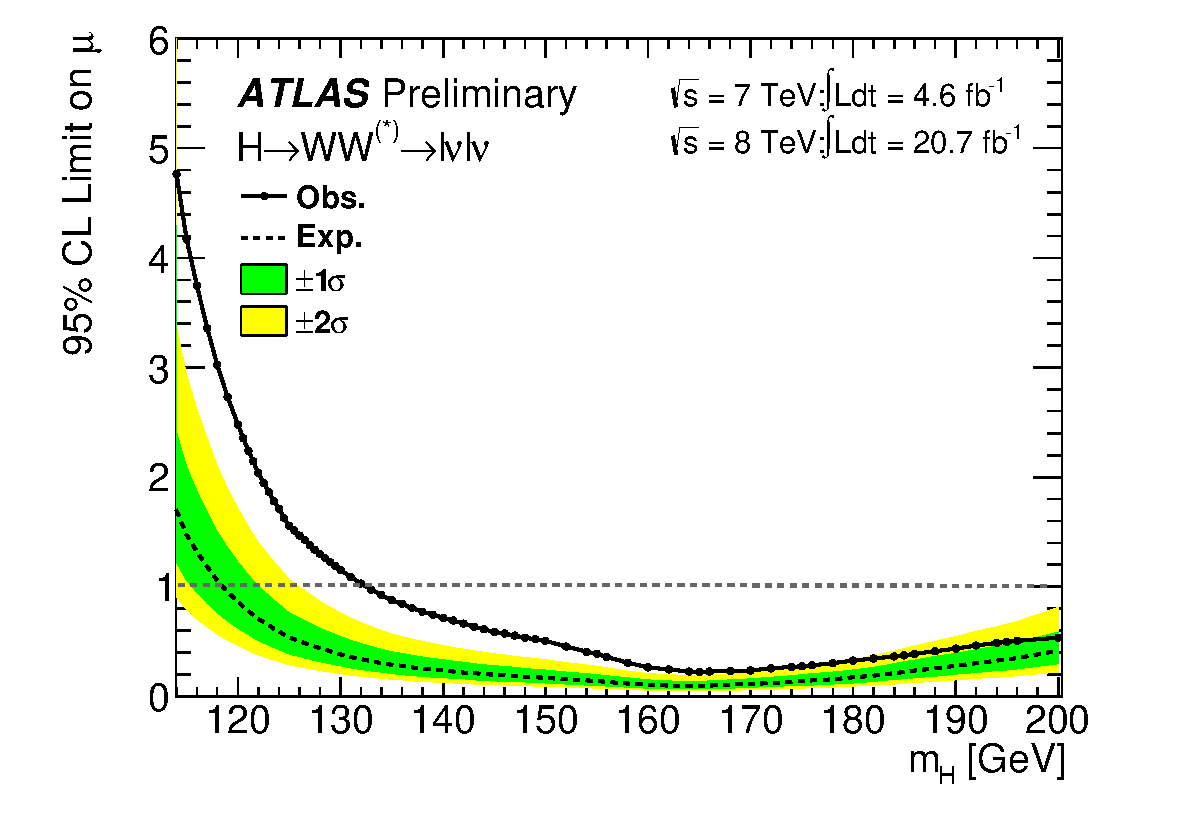
\includegraphics[width=\textwidth]{tex/results/Mor13_CLs}
		\caption{Exclusion}
		\label{fig:results:CLs}
	\end{subfigure}
	\hfill
	\begin{subfigure}[b]{0.495\textwidth}
		\centering
		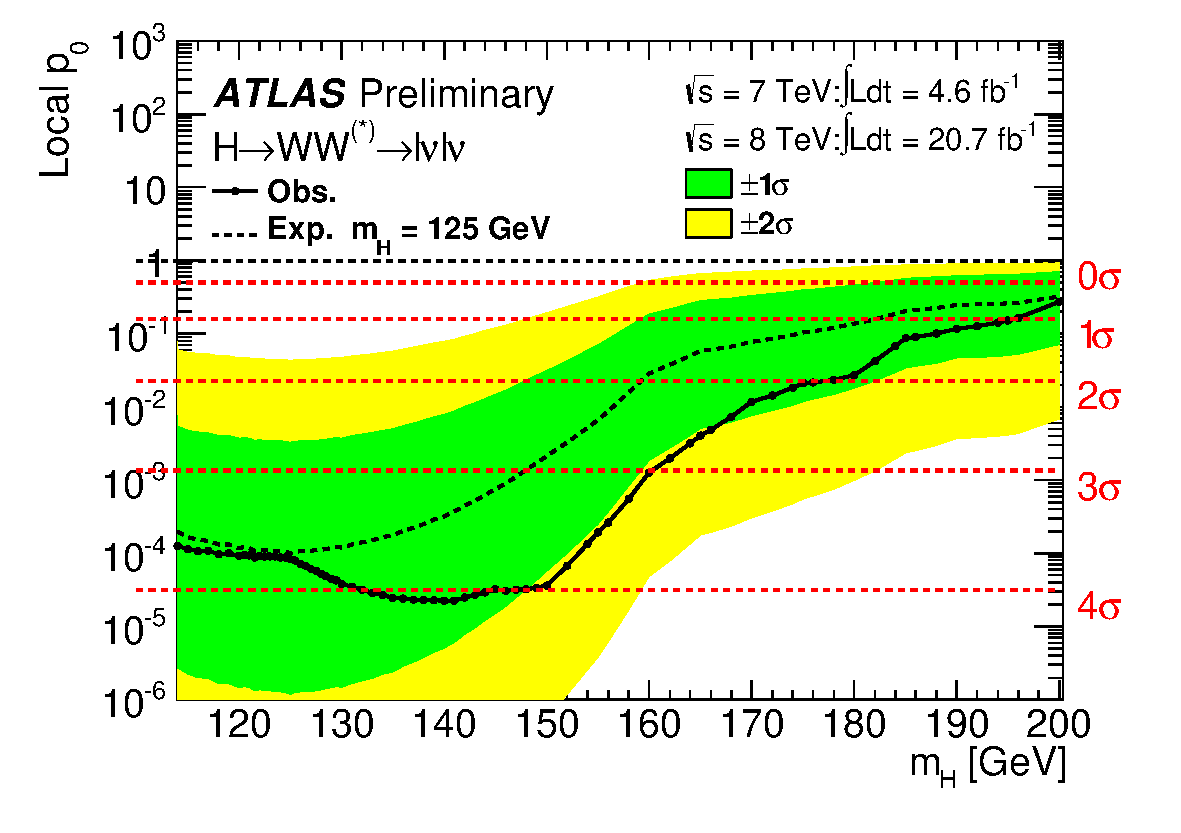
\includegraphics[width=\textwidth]{tex/results/Mor13_p0}
		\caption{Discovery}
		\label{fig:results:p0}
	\end{subfigure}
	\caption{(a) The observed (solid) 95\% CL upper limit on the signal strength $\mu$ as a 
	function of \mH and the expectation (dashed) under the background-only hypothesis. \\
	(b) The observed (solid) $p_0$ as a function of \mH and the expectation (dashed) under 
	the signal-plus-background hypothesis with \unit{$\mH = 125$}{\GeV} and $\mu = 1$.
	The bands show the $\pm1\sigma$ and $\pm2\sigma$ uncertainties on the expectation.}
\end{figure}

The measured signal strength $\hat{\mu}$ as a function of the \mH under test is shown in 
\Figure~\ref{fig:results:mu}. A broad range of Higgs boson masses are consistent with the 
assumption that the Higgs boson behaves as predicted by the SM (\ie $\mu = 1$). The data are 
also consistent with a lower mass Higgs boson with $\mu > 1$ or a higher mass Higgs boson 
with $\mu < 1$. By including \mH as a parameter of interest in the fit, it is possible to 
test which $\parenths{\mu, \mH}$ pair are most favoured by the data. This is presented in 
\Figure~\ref{fig:results:mu_mH}, together with the 68\% CL and 95\% CL contours. This 
clearly demonstrates that the analysis is more sensitive to $\mu$ than to \mH.

\begin{figure}[t]
	\begin{subfigure}[b]{0.495\textwidth}
		\centering
		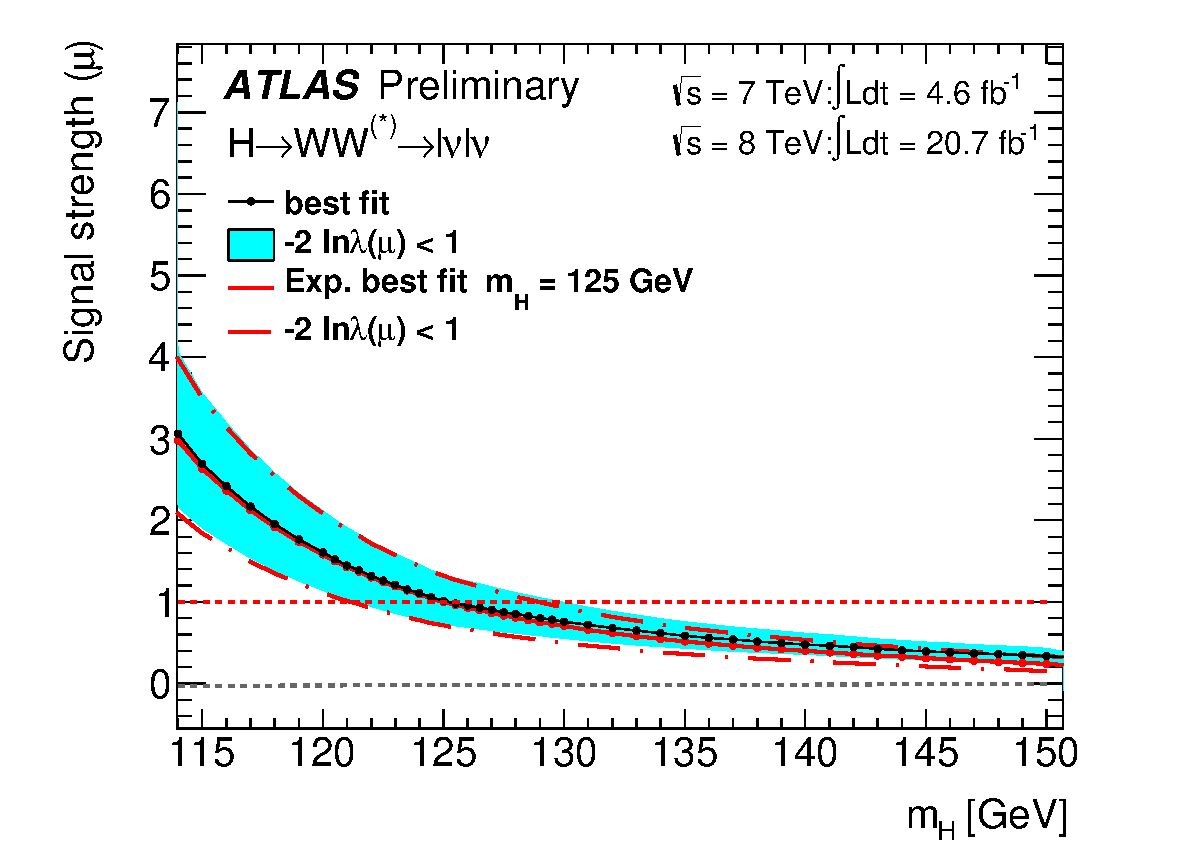
\includegraphics[width=\textwidth]{tex/results/Mor13_mu}
		\caption{Measurement of $\mu$}
		\label{fig:results:mu}
	\end{subfigure}
	\hfill
	\begin{subfigure}[b]{0.495\textwidth}
		\centering
		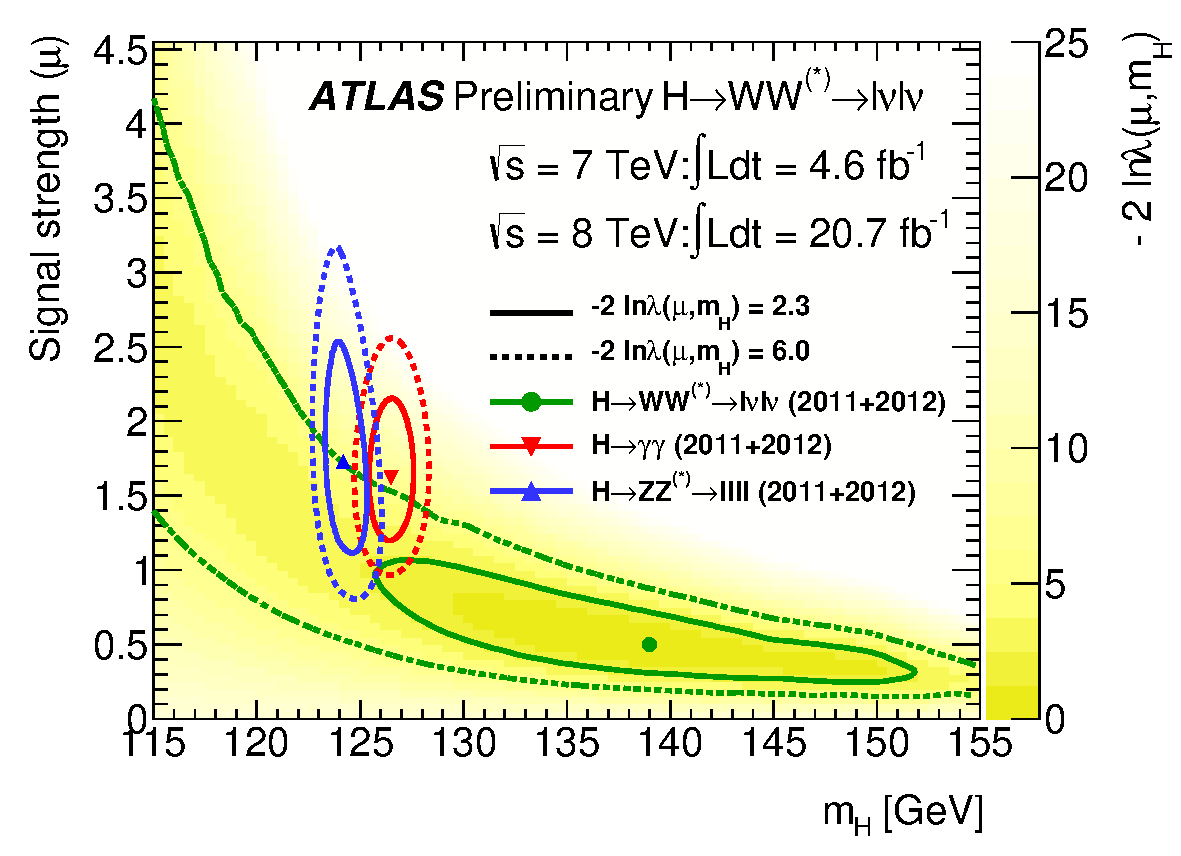
\includegraphics[width=\textwidth]{tex/results/Mor13_mu_mH}
		\caption{Measurement of $\parenths{\mu, \mH}$}
		\label{fig:results:mu_mH}
	\end{subfigure}
	\caption{(a) The best-fit signal strength $\hat{\mu}$ (solid) as a function of \mH, with 
	the 68\% CL interval shown. (b) The best-fit signal strength $\hat{\mu}$ and mass 
	$\hat{m}_{\PHiggs}$ (marker), with the 68\% CL and 95\% CL intervals shown.}
\end{figure}

The above results exhibit more than $5\sigma$ significance for the \ggHWWlvlv process, and 
consequently for the existence of the Higgs boson itself. LHC searches for 
\HepProcess{\PHiggs \HepTo \Pphoton\Pphoton} and \HepProcess{\PHiggs \HepTo \PZ\PZ} have 
found consistent evidence, which is summarised in \Section~\ref{sec:searches}. These two 
channels yield much better mass sensitivity, and observe \unit{$\mH \approx 125$}{\GeV}. 
For this reason, the above results are now reinterpreted in terms of a Higgs boson with 
\unit{$\mH = 125$}{\GeV}.

With \unit{$\mH = 125$}{\GeV}, the observed significance is $5.3\sigma$ and the expected 
significance is $5.0\sigma$. The measured signal strength is $\hat{\mu} = 1.14 \pm 0.28$. 
The significance and $\hat{\mu}$ observed in various signal regions are summarised in 
\Table~\ref{tab:results:sig_mu_breakdown}. This shows that the combined observation is 
mostly driven by the \emch and \mech channels of the 0-jet and 1-jet bins, in the 
\unit{$\sqrt{s} = 8$}{\TeV} dataset.

\begin{table}
	\begin{tabular}{l@{\hskip 0.4in}cc@{\hskip 0.4in}cc}
		\toprule
		& \multicolumn{2}{c@{\hskip 0.4in}}{\unit{$\sqrt{s} = 7$}{\TeV}} & \multicolumn{2}{c}{\unit{$\sqrt{s} = 8$}{\TeV}} \\
		& $Z_{\text{obs}}$ ($Z_{\text{exp}}$) & $\hat{\mu}_{\text{obs}}$ & $Z_{\text{obs}}$ ($Z_{\text{exp}}$) & $\hat{\mu}_{\text{obs}}$ \\
		\midrule
		Total                    & 1.8 (1.8) & $0.99^{+0.00}_{-0.00}$ & 4.9 (4.4) & $1.18^{+0.31}_{-0.27}$ \\
		\quad 0-jet              & 1.2 (1.5) & $0.75^{+0.00}_{-0.00}$ & 4.2 (3.6) & $1.26^{+0.42}_{-0.35}$ \\
		\quad\quad \emch{}+\mech & 0.9 (1.4) & $0.61^{+0.00}_{-0.00}$ & 4.4 (3.6) & $1.41^{+0.45}_{-0.38}$ \\
		\quad\quad \eech{}+\mmch & 1.0 (0.7) & $1.40^{+0.00}_{-0.00}$ & 0.2 (1.2) & $0.18^{+0.83}_{-0.77}$ \\
		\quad 1-jet              & 1.8 (1.1) & $1.70^{+0.00}_{-0.00}$ & 2.5 (2.5) & $1.02^{+0.52}_{-0.43}$ \\
		\quad\quad \emch{}+\mech & 2.0 (1.0) & $2.20^{+0.00}_{-0.00}$ & 2.8 (2.5) & $1.21^{+0.57}_{-0.46}$ \\
		\quad\quad \eech{}+\mmch & 0.1 (0.6) & $0.17^{+0.00}_{-0.00}$ & 0.4 (1.0) & $0.38^{+1.09}_{-1.04}$ \\
		\quad \twojet            & --        & --                     & 1.4 (1.2) & $1.22^{+0.96}_{-0.85}$ \\
		\bottomrule
	\end{tabular}
	\caption{The observed and expected significances in units of Gaussian standard 
	deviations, $Z$, and the measured signal strength for a Higgs boson with 
	\unit{$\mH = 125$}{\GeV}.}
	\label{tab:results:sig_mu_breakdown}
\end{table}

%Table of uncertainties on $\mu$





% \subsection{Cross section measurements}
% \label{sec:results:xs}

% introduce observed resonance at mH = 125 GeV
% mu @ 125 
% measured total cross section
% split mu into jet bins
% measured fiducial cross sections
